\documentclass[8pt,aspectratio=169]{beamer}
\usetheme{Madrid}
\usepackage{graphicx}
\usepackage{booktabs}
\usepackage{adjustbox}
\usepackage{multicol}
\usepackage{amsmath}
\usepackage{amssymb}
\usepackage{tikz}
\usepackage{hyperref}
\usepackage{algorithm}
\usepackage{algorithmic}
\usepackage{colortbl}
\usepackage{pgfplots}
\pgfplotsset{compat=1.18}

% TikZ libraries for comics, diagrams, stakeholder maps
\usetikzlibrary{arrows.meta,positioning,shapes.callouts,shapes.geometric,decorations.pathreplacing}

% Color definitions
\definecolor{mlblue}{RGB}{0,102,204}
\definecolor{mlpurple}{RGB}{51,51,178}
\definecolor{mllavender}{RGB}{173,173,224}
\definecolor{mllavender2}{RGB}{193,193,232}
\definecolor{mllavender3}{RGB}{204,204,235}
\definecolor{mllavender4}{RGB}{214,214,239}
\definecolor{mlorange}{RGB}{255, 127, 14}
\definecolor{mlgreen}{RGB}{44, 160, 44}
\definecolor{mlred}{RGB}{214, 39, 40}
\definecolor{mlgray}{RGB}{127, 127, 127}
\definecolor{lightgray}{RGB}{240, 240, 240}
\definecolor{midgray}{RGB}{180, 180, 180}

% NEW COLORS for mini-lecture
\definecolor{dfteal}{RGB}{0,128,128}
\definecolor{dfred}{RGB}{180,30,30}

% Backward compatibility
\colorlet{MLPurple}{mlpurple}
\colorlet{MLBlue}{mlblue}
\colorlet{MLOrange}{mlorange}
\colorlet{MLGreen}{mlgreen}
\colorlet{MLRed}{mlred}
\colorlet{MLLavender}{mllavender}
\colorlet{MLGray}{mlgray}

% Theme colors (exact Madrid settings)
\setbeamercolor{palette primary}{bg=mllavender3,fg=mlpurple}
\setbeamercolor{palette secondary}{bg=mllavender2,fg=mlpurple}
\setbeamercolor{palette tertiary}{bg=mllavender,fg=white}
\setbeamercolor{palette quaternary}{bg=mlpurple,fg=white}
\setbeamercolor{structure}{fg=mlpurple}
\setbeamercolor{section in toc}{fg=mlpurple}
\setbeamercolor{subsection in toc}{fg=mlblue}
\setbeamercolor{title}{fg=mlpurple}
\setbeamercolor{frametitle}{fg=mlpurple,bg=mllavender3}
\setbeamercolor{block title}{bg=mllavender2,fg=mlpurple}
\setbeamercolor{block body}{bg=mllavender4,fg=black}
\setbeamertemplate{navigation symbols}{}
\setbeamertemplate{itemize items}[circle]
\setbeamertemplate{enumerate items}[default]
\setbeamersize{text margin left=5mm,text margin right=5mm}

% Footer
\setbeamertemplate{footline}{
  \leavevmode%
  \hbox{%
    \begin{beamercolorbox}[wd=.333333\paperwidth,ht=2.25ex,dp=1ex,center]{author in head/foot}%
      \usebeamerfont{author in head/foot}Methods and Algorithms
    \end{beamercolorbox}%
    \begin{beamercolorbox}[wd=.333333\paperwidth,ht=2.25ex,dp=1ex,center]{title in head/foot}%
      \usebeamerfont{title in head/foot}MSc Data Science
    \end{beamercolorbox}%
    \begin{beamercolorbox}[wd=.333333\paperwidth,ht=2.25ex,dp=1ex,right]{date in head/foot}%
      \usebeamerfont{date in head/foot}\insertframenumber{} / \inserttotalframenumber\hspace*{2ex}
    \end{beamercolorbox}}%
  \vskip0pt%
}

\newcommand{\bottomnote}[1]{%
\vfill
\vspace{-2mm}
\textcolor{mllavender2}{\rule{\textwidth}{0.4pt}}
\vspace{1mm}
\footnotesize
\textbf{#1}
}

\newenvironment{compactlist}{%
  \begin{itemize}%
    \setlength{\itemsep}{2pt}%
    \setlength{\parskip}{0pt}%
    \setlength{\parsep}{0pt}%
}{%
  \end{itemize}%
}

\newcommand{\highlight}[1]{\textcolor{mlorange}{\textbf{#1}}}
\newcommand{\mathbold}[1]{\boldsymbol{#1}}

\title[K-Means Mini-Lecture]{K-Means Clustering}
\subtitle{A 10-Slide Mini-Lecture}
\author{Methods and Algorithms}
\institute{MSc Data Science}
\date{}

\begin{document}

%% ================================================================
%% SLIDE 1: WHY -- TikZ Comic (Dilemma)
%% ================================================================
\begin{frame}[t]
\frametitle{Why Would a Marketing Team Want to Group Customers Without Labels?}
\begin{columns}[T]
\begin{column}{0.55\textwidth}
\small
\textbf{The Dilemma}
\begin{compactlist}
\item A bank has thousands of customers but no predefined categories
\item Management asks ``which customers are similar?'' but nobody agrees
\item The data has patterns but nobody labeled them
\end{compactlist}

\vspace{2mm}
What if the structure is already in the data -- waiting to be discovered?

\begin{block}{Insight}
K-Means formalizes unsupervised discovery: let the algorithm find groups that the data itself defines, rather than imposing human categories.
\end{block}
\end{column}

\begin{column}{0.42\textwidth}
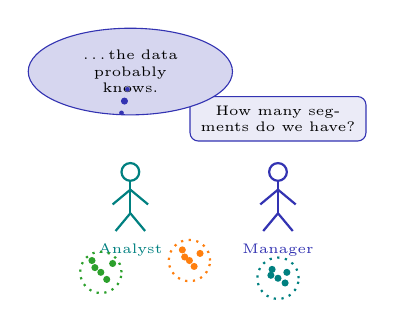
\begin{tikzpicture}[scale=0.75]
% Analyst stick figure
\draw[dfteal, thick] (1,2.1) circle (0.15);
\draw[dfteal, thick] (1,1.95) -- (1,1.4);
\draw[dfteal, thick] (1,1.8) -- (0.7,1.55);
\draw[dfteal, thick] (1,1.8) -- (1.3,1.55);
\draw[dfteal, thick] (1,1.4) -- (0.75,1.1);
\draw[dfteal, thick] (1,1.4) -- (1.25,1.1);
\node[dfteal, below, font=\tiny] at (1,1.05) {Analyst};
% Manager stick figure
\draw[mlpurple, thick] (3.5,2.1) circle (0.15);
\draw[mlpurple, thick] (3.5,1.95) -- (3.5,1.4);
\draw[mlpurple, thick] (3.5,1.8) -- (3.2,1.55);
\draw[mlpurple, thick] (3.5,1.8) -- (3.8,1.55);
\draw[mlpurple, thick] (3.5,1.4) -- (3.25,1.1);
\draw[mlpurple, thick] (3.5,1.4) -- (3.75,1.1);
\node[mlpurple, below, font=\tiny] at (3.5,1.05) {Manager};
% Manager speech bubble
\node[draw=mlpurple, fill=mlpurple!10, rounded corners=3pt,
      font=\tiny, text width=2.0cm, align=center]
      at (3.5,3.0) {How many segments do we have?};
% Analyst thought bubble
\node[draw=mlpurple, fill=mllavender4, ellipse,
      font=\tiny, text width=1.6cm, align=center]
      at (1.0,3.8) {\ldots the data probably knows.};
\fill[mlpurple] (0.85,3.1) circle (0.04);
\fill[mlpurple] (0.9,3.3) circle (0.06);
\fill[mlpurple] (0.95,3.5) circle (0.04);
% Three clusters of dots below
\foreach \dx/\dy in {0/0, 0.2/0.15, -0.15/0.2, 0.1/-0.12, -0.1/0.08} {
  \fill[mlgreen] ({0.5+\dx}, {0.4+\dy}) circle (0.06);
}
\foreach \dx/\dy in {0/0, 0.18/0.12, -0.12/0.18, 0.08/-0.1, -0.08/0.06} {
  \fill[mlorange] ({2.0+\dx}, {0.6+\dy}) circle (0.06);
}
\foreach \dx/\dy in {0/0, 0.15/0.1, -0.1/0.15, 0.12/-0.08, -0.12/0.05} {
  \fill[dfteal] ({3.5+\dx}, {0.3+\dy}) circle (0.06);
}
\draw[dotted, mlgreen, thick] (0.5,0.4) circle (0.35);
\draw[dotted, mlorange, thick] (2.0,0.6) circle (0.35);
\draw[dotted, dfteal, thick] (3.5,0.3) circle (0.35);
\end{tikzpicture}
\end{column}
\end{columns}

\bottomnote{Unsupervised learning finds structure without labels -- the algorithm discovers categories, not confirms them}
\end{frame}

%% ================================================================
%% SLIDE 2: FEEL -- Text-Only with Prompt
%% ================================================================
\begin{frame}[t]
\frametitle{Sorting a Crowd -- Did Clustering Cross Your Mind?}
\begin{columns}[T]
\begin{column}{0.55\textwidth}
\small
\textbf{Think Before You Compute}

\footnotesize
Imagine you are at a networking event with a hundred strangers. Within minutes, you mentally group people: the tech crowd near the coffee, the finance professionals by the window, the academics clustered around the speaker. You did not run an algorithm. You noticed patterns.

\begin{compactlist}
\item How many groups did you identify?
\item What features separated them -- dress, language, location?
\item Did some people seem to belong to two groups at once?
\end{compactlist}

\begin{exampleblock}{Reflection Prompt}
Write down one situation where you mentally grouped items or people without being told the categories. How many clusters did you find?
\end{exampleblock}
\end{column}

\begin{column}{0.42\textwidth}
\footnotesize
\vspace{4mm}
\fcolorbox{mlpurple}{mllavender4}{\parbox{0.85\columnwidth}{%
\textbf{Pause and reflect:}

\vspace{2mm}
When you last organized files on your desktop, did you sort them into folders based on perceived similarity -- without anyone telling you the folder names?

\vspace{2mm}
\textbf{That is clustering.}
}}
\end{column}
\end{columns}

\bottomnote{Clustering mirrors how humans naturally organize: by perceived similarity, not by assigned labels}
\end{frame}

%% ================================================================
%% SLIDE 3: WHAT -- Comparison Table
%% ================================================================
\begin{frame}[t]
\frametitle{What Makes K-Means Different from DBSCAN, Hierarchical, and GMM?}
\begin{columns}[T]
\begin{column}{0.55\textwidth}
\small
\textbf{Taxonomy of Clustering Algorithms}

\vspace{1mm}
\footnotesize
\begin{tabular}{@{}l c c c c@{}}
\toprule
\textbf{Property} & \textbf{\textcolor{dfteal}{K-M}} & \textbf{DBS} & \textbf{Hier.} & \textbf{GMM} \\
\midrule
\rowcolor{mllavender4}
Choose K & Yes & No & Cut & Yes \\
Shape & Spher. & Arb. & Any & Ellip. \\
\rowcolor{mllavender4}
Outliers & All & Det. & All & Soft \\
Speed & $nKt$ & $n\!\log\!n$ & $n^2$ & $nK$ \\
\rowcolor{mllavender4}
Output & Hard & Hard+ & Dend. & Soft \\
\bottomrule
\end{tabular}

\vspace{2mm}
\scriptsize\textbf{K-Means is the fastest and simplest, but assumes spherical clusters and assigns every point.}

\begin{block}{Insight}
\scriptsize K-Means wins on speed and simplicity but pays a price: it cannot discover non-spherical clusters or flag outliers.
\end{block}
\end{column}

\begin{column}{0.42\textwidth}
\footnotesize
\vspace{2mm}
\colorbox{dfteal!15}{\parbox{0.9\columnwidth}{\textbf{K-Means:} Fast, spherical, hard}}

\vspace{3mm}
\colorbox{mlorange!15}{\parbox{0.9\columnwidth}{\textbf{DBSCAN:} Density, arbitrary shape}}

\vspace{3mm}
\colorbox{mlpurple!15}{\parbox{0.9\columnwidth}{\textbf{Hierarchical:} Tree, any K post-hoc}}

\vspace{3mm}
\colorbox{mlgreen!15}{\parbox{0.9\columnwidth}{\textbf{GMM:} Probabilistic, soft assign}}
\end{column}
\end{columns}

\bottomnote{Spherical assumption means K-Means minimizes within-cluster variance, equivalent to Voronoi tessellation}
\end{frame}

%% ================================================================
%% SLIDE 4: CASE -- Step Diagram / Timeline
%% ================================================================
\begin{frame}[t]
\frametitle{Follow One Iteration from Random Centers to Stable Clusters}
\begin{columns}[T]
\begin{column}{0.55\textwidth}
\small
\textbf{One Iteration, Step by Step}
\begin{compactlist}
\item Start with K random centroids
\item Assign every point to nearest centroid (Voronoi partition)
\item Recompute each centroid as the mean of its assigned points
\item Repeat until centroids stop moving
\item Convergence guaranteed: each step reduces WCSS
\end{compactlist}

\begin{block}{Insight}
\scriptsize K-Means always converges, but to a local minimum -- not necessarily the global one.
\end{block}
\end{column}

\begin{column}{0.42\textwidth}
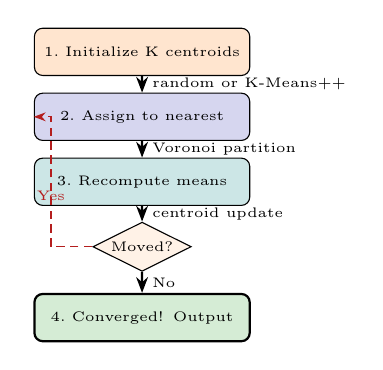
\begin{tikzpicture}[scale=0.75,
  stepnode/.style={draw, rounded corners=3pt, font=\tiny,
    text width=2.5cm, align=center, minimum height=0.6cm},
  arr/.style={-{Stealth[length=2mm]}, thick}]
% Nodes
\node[stepnode, fill=mlorange!20] (s1) at (1.5,5.0)
  {1.\ Initialize K centroids};
\node[stepnode, fill=mllavender4] (s2) at (1.5,3.9)
  {2.\ Assign to nearest};
\node[stepnode, fill=dfteal!20] (s3) at (1.5,2.8)
  {3.\ Recompute means};
% Decision diamond
\node[draw, diamond, fill=mlorange!10, font=\tiny,
      inner sep=1pt, aspect=2] (dec) at (1.5,1.7) {Moved?};
% Final node
\node[stepnode, fill=mlgreen!20, thick] (s4) at (1.5,0.5)
  {4.\ Converged! Output};
% Arrows with labels
\draw[arr] (s1) -- (s2)
  node[midway, right, font=\tiny] {random or K-Means++};
\draw[arr] (s2) -- (s3)
  node[midway, right, font=\tiny] {Voronoi partition};
\draw[arr] (s3) -- (dec)
  node[midway, right, font=\tiny] {centroid update};
\draw[arr] (dec) -- (s4)
  node[midway, right, font=\tiny] {No};
% Yes: loop back
\draw[-{Stealth[length=1.5mm]}, dfred, densely dashed]
  (dec.west) -- +(-0.7,0) |- (s2.west)
  node[pos=0.25, below, font=\tiny] {Yes};
\end{tikzpicture}
\end{column}
\end{columns}

\bottomnote{Each iteration is O(nKd): n points, K clusters, d dimensions. Typically converges in few iterations.}
\end{frame}

%% ================================================================
%% SLIDE 5: HOW -- Side-by-Side Architecture
%% ================================================================
\begin{frame}[t]
\frametitle{Who Should Pick the Starting Centers -- Random, K-Means++, or Both?}
\begin{columns}[T]
\begin{column}{0.55\textwidth}
\small
\textbf{Three Initialization Strategies}
\begin{compactlist}
\item \textbf{Random}: pick K points at random, fast but high variance
\item \textbf{K-Means++}: distance-proportional sampling, spreads centers apart
\item \textbf{Multiple restarts}: run R times, keep the run with lowest WCSS
\end{compactlist}

\vspace{1mm}
\scriptsize K-Means++ is now the default in scikit-learn for good reason.

\begin{block}{Insight}
\scriptsize K-Means++ initialization reduces both the expected WCSS and the number of iterations.
\end{block}
\end{column}

\begin{column}{0.42\textwidth}
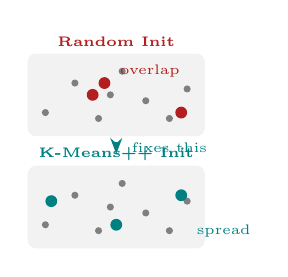
\begin{tikzpicture}[scale=0.75]
% -- Top: Random Init --
\node[font=\tiny\bfseries, dfred] at (1.5,4.8) {Random Init};
\fill[mlgray!10, rounded corners=3pt] (0,3.2) rectangle (3.0,4.6);
% Data points
\foreach \px/\py in {0.3/3.6, 0.8/4.1, 1.2/3.5, 1.6/4.3,
  2.0/3.8, 2.4/3.5, 2.7/4.0, 1.4/3.9} {
  \fill[mlgray] (\px,\py) circle (0.06);
}
% Two close centroids + one spread
\fill[dfred] (1.1,3.9) circle (0.1);
\fill[dfred] (1.3,4.1) circle (0.1);
\fill[dfred] (2.6,3.6) circle (0.1);
\node[font=\tiny, dfred, right] at (1.4,4.3) {overlap};
% -- Bottom: K-Means++ Init --
\node[font=\tiny\bfseries, dfteal] at (1.5,2.9) {K-Means++ Init};
\fill[mlgray!10, rounded corners=3pt] (0,1.3) rectangle (3.0,2.7);
% Same data layout
\foreach \px/\py in {0.3/1.7, 0.8/2.2, 1.2/1.6, 1.6/2.4,
  2.0/1.9, 2.4/1.6, 2.7/2.1, 1.4/2.0} {
  \fill[mlgray] (\px,\py) circle (0.06);
}
% Well-spread centroids
\fill[dfteal] (0.4,2.1) circle (0.1);
\fill[dfteal] (1.5,1.7) circle (0.1);
\fill[dfteal] (2.6,2.2) circle (0.1);
\node[font=\tiny, dfteal, right] at (2.7,1.6) {spread};
% Arrow between
\draw[-{Stealth[length=2mm]}, dfteal, thick]
  (1.5,3.1) -- (1.5,2.9);
\node[font=\tiny, dfteal, right] at (1.6,3.0) {fixes this};
\end{tikzpicture}
\end{column}
\end{columns}

\bottomnote{K-Means++ guarantees O(log K)-competitive approximation to optimal WCSS (Arthur and Vassilvitskii)}
\end{frame}

%% ================================================================
%% SLIDE 6: RISK -- TikZ Comic (Failure)
%% ================================================================
\begin{frame}[t]
\frametitle{What Could Go Wrong If You Choose the Wrong K?}
\begin{columns}[T]
\begin{column}{0.55\textwidth}
\small
\textbf{Three Ways K-Means Fails Silently}
\begin{compactlist}
\item \textbf{Wrong K}: too few clusters merge real groups, too many split them
\item \textbf{Non-spherical data}: K-Means forces round clusters on curved structure
\item \textbf{Bad initialization}: trapped in a poor local minimum with high WCSS
\end{compactlist}

\begin{block}{Insight}
\scriptsize K-Means always finds K clusters, even when the true number is different. The algorithm never says ``I don't know.''
\end{block}
\end{column}

\begin{column}{0.42\textwidth}
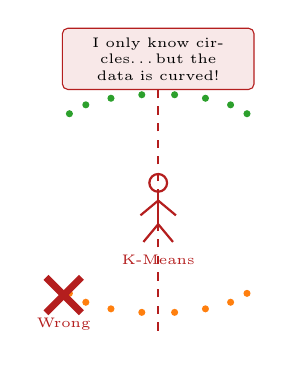
\begin{tikzpicture}[scale=0.75]
% K-Means stick figure in center
\draw[dfred, thick] (2.5,2.5) circle (0.15);
\draw[dfred, thick] (2.5,2.35) -- (2.5,1.8);
\draw[dfred, thick] (2.5,2.2) -- (2.2,1.95);
\draw[dfred, thick] (2.5,2.2) -- (2.8,1.95);
\draw[dfred, thick] (2.5,1.8) -- (2.25,1.5);
\draw[dfred, thick] (2.5,1.8) -- (2.75,1.5);
\node[dfred, below, font=\tiny] at (2.5,1.45) {K-Means};
% Upper arc of dots (mlgreen)
\foreach \angle in {20,40,60,80,100,120,140,160} {
  \fill[mlgreen] ({2.5+1.6*cos(\angle)}, {3.5+0.5*sin(\angle)}) circle (0.06);
}
% Lower arc of dots (mlorange)
\foreach \angle in {200,220,240,260,280,300,320,340} {
  \fill[mlorange] ({2.5+1.6*cos(\angle)}, {0.8+0.5*sin(\angle)}) circle (0.06);
}
% Wrong vertical split line
\draw[dfred, thick, dashed] (2.5,0.0) -- (2.5,4.2);
% Speech bubble
\node[draw=dfred, fill=dfred!10, rounded corners=2pt,
      font=\tiny, text width=2.2cm, align=center]
      at (2.5,4.6) {I only know circles\ldots but the data is curved!};
% Large X
\draw[dfred, line width=2.5pt] (0.6,0.3) -- (1.2,0.9);
\draw[dfred, line width=2.5pt] (0.6,0.9) -- (1.2,0.3);
\node[font=\tiny, dfred] at (0.9,0.1) {Wrong};
\end{tikzpicture}
\end{column}
\end{columns}

\bottomnote{Diagnostics: elbow method for K, silhouette score for cluster quality, visual inspection for shape assumptions}
\end{frame}

%% ================================================================
%% SLIDE 7: WHERE -- External Chart (PDF)
%% ================================================================
\begin{frame}[t]
\frametitle{Why Do So Many Practitioners Reach for K-Means First?}
\begin{columns}[T]
\begin{column}{0.55\textwidth}
\small
\textbf{K-Means as a Baseline Clusterer}
\begin{compactlist}
\item Scales linearly with data size
\item Simple to implement, explain, and debug
\item Results easy to interpret: each cluster has a centroid
\item Natural starting point before complex alternatives
\end{compactlist}

\vspace{1mm}
\scriptsize The chart shows how cluster boundaries emerge from the iteration process.

\begin{block}{Insight}
\scriptsize K-Means owes its popularity to the same property as linear regression: the simplest reasonable solution, making it the natural baseline.
\end{block}
\end{column}

\begin{column}{0.42\textwidth}
\vspace{2mm}
\includegraphics[width=\textwidth]{03_kmeans_iteration/chart.pdf}
\end{column}
\end{columns}

\bottomnote{K-Means with K=2 is equivalent to finding the optimal split along the first principal component direction}
\end{frame}

%% ================================================================
%% SLIDE 8: IMPACT -- Stakeholder Map
%% ================================================================
\begin{frame}[t]
\frametitle{Who Wins and Who Loses When Clusters Replace Categories?}
\begin{columns}[T]
\begin{column}{0.55\textwidth}
\small
\textbf{Stakeholder Analysis}
\begin{compactlist}
\item \textbf{Winners}: Marketing (data-driven segments), Fraud detection (anomaly = far from centroids), Data preprocessing (cluster features)
\item \textbf{Losers}: Domain experts (categories overridden), Interpretability advocates, Anyone expecting stable segments over time
\end{compactlist}

\vspace{1mm}
\scriptsize K-Means shifts power from domain intuition to data patterns.

\begin{block}{Insight}
\scriptsize K-Means clusters are not ``real'' categories -- they are mathematical artifacts. The business meaning must be assigned after.
\end{block}
\end{column}

\begin{column}{0.42\textwidth}
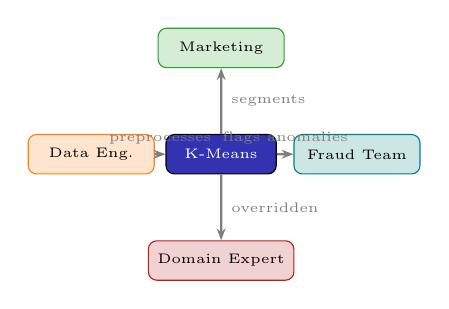
\begin{tikzpicture}[scale=0.75,
  actor/.style={draw, rounded corners=3pt, font=\tiny,
    minimum width=1.6cm, minimum height=0.5cm, align=center},
  arr/.style={-{Stealth[length=1.5mm]}, thick, mlgray}]
% Center
\node[actor, fill=mlpurple, text=white, minimum width=1.4cm]
  (km) at (2.2,2.2) {K-Means};
% Top: Marketing
\node[actor, fill=mlgreen!20, draw=mlgreen]
  (mkt) at (2.2,4.0) {Marketing};
\draw[arr] (km) -- (mkt)
  node[midway, right, font=\tiny] {segments};
% Right: Fraud Team
\node[actor, fill=dfteal!20, draw=dfteal]
  (fraud) at (4.5,2.2) {Fraud Team};
\draw[arr] (km) -- (fraud)
  node[midway, above, font=\tiny] {flags anomalies};
% Bottom: Domain Expert
\node[actor, fill=dfred!20, draw=dfred]
  (dom) at (2.2,0.4) {Domain Expert};
\draw[arr] (km) -- (dom)
  node[midway, right, font=\tiny] {overridden};
% Left: Data Eng.
\node[actor, fill=mlorange!20, draw=mlorange]
  (eng) at (0,2.2) {Data Eng.};
\draw[arr] (eng) -- (km)
  node[midway, above, font=\tiny] {preprocesses};
\end{tikzpicture}
\end{column}
\end{columns}

\bottomnote{Cluster interpretation requires domain expertise: the algorithm finds groups, humans name them}
\end{frame}

%% ================================================================
%% SLIDE 9: SO WHAT -- Metaphor Visual (Balance Scale)
%% ================================================================
\begin{frame}[t]
\frametitle{3 Questions That Reveal Whether K-Means Is the Right Algorithm}
\begin{columns}[T]
\begin{column}{0.55\textwidth}
\small
\textbf{The Decision Framework}
\begin{enumerate}
\setlength{\itemsep}{2pt}
\item \textbf{Are clusters spherical?} -- If not, consider DBSCAN or spectral clustering
\item \textbf{Do you know how many clusters?} -- If not, try elbow, silhouette, or hierarchical
\item \textbf{Every point in exactly one group?} -- If overlap needed, use GMM
\end{enumerate}

\vspace{1mm}
\scriptsize If all three answers are yes, K-Means is a strong candidate.

\begin{block}{Insight}
\scriptsize No clustering algorithm is universally best. K-Means excels on spherical, well-separated clusters with known K.
\end{block}
\end{column}

\begin{column}{0.42\textwidth}
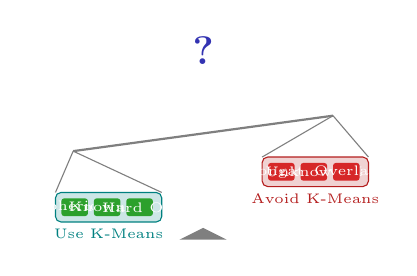
\begin{tikzpicture}[scale=0.75]
% Fulcrum
\fill[mlgray] (2.5,0.2) -- (2.1,0) -- (2.9,0) -- cycle;
% Beam (tilted: left lower = Use K-Means)
\draw[thick, mlgray] (0.3,1.5) -- (4.7,2.1);
% Left pan: Use K-Means
\draw[mlgray] (0.3,1.5) -- (0.0,0.8);
\draw[mlgray] (0.3,1.5) -- (1.8,0.8);
\draw[dfteal, fill=dfteal!20, rounded corners=2pt]
  (0.0,0.3) rectangle (1.8,0.8);
\foreach \i/\txt in {0/Spherical, 1/Known K, 2/Hard OK} {
  \fill[mlgreen, rounded corners=1pt]
    ({0.1+\i*0.55}, 0.4) rectangle ({0.55+\i*0.55}, 0.7);
  \node[font=\tiny, white] at ({0.33+\i*0.55}, 0.55) {\txt};
}
\node[font=\tiny, dfteal] at (0.9,0.1) {Use K-Means};
% Right pan: Avoid K-Means
\draw[mlgray] (4.7,2.1) -- (3.5,1.4);
\draw[mlgray] (4.7,2.1) -- (5.3,1.4);
\draw[dfred, fill=dfred!20, rounded corners=2pt]
  (3.5,0.9) rectangle (5.3,1.4);
\foreach \i/\txt in {0/Elongated, 1/Unknown K, 2/Overlap} {
  \fill[mlred, rounded corners=1pt]
    ({3.6+\i*0.55}, 1.0) rectangle ({4.05+\i*0.55}, 1.3);
  \node[font=\tiny, white] at ({3.83+\i*0.55}, 1.15) {\txt};
}
\node[font=\tiny, dfred] at (4.4,0.7) {Avoid K-Means};
% Question mark
\node[mlpurple, font=\Large\bfseries] at (2.5,3.2) {?};
\end{tikzpicture}
\end{column}
\end{columns}

\bottomnote{The ``No Free Lunch'' theorem applies to clustering too: no single algorithm dominates all data shapes}
\end{frame}

%% ================================================================
%% SLIDE 10: ACT -- Activity Frame
%% ================================================================
\begin{frame}[t]
\frametitle{Can You Evaluate This Real Clustering Problem?}
\begin{columns}[T]
\begin{column}{0.55\textwidth}
\small
\textbf{The Scenario}

\footnotesize
A retail bank wants to segment its customers. Features: income, transaction amount, transaction count, tenure, credit utilization. All numerical, no predefined categories.

\begin{compactlist}
\item Apply the 3-question framework from the previous slide
\item Decide: Is K-Means appropriate here?
\item If yes: recommend K and a validation strategy
\item If no: name a better algorithm and explain why
\end{compactlist}

\begin{exampleblock}{Deliverable}
\scriptsize Fill in the table. Be prepared to defend your verdict to a skeptical marketing director.
\end{exampleblock}
\end{column}

\begin{column}{0.42\textwidth}
\footnotesize
\vspace{2mm}
\begin{tabular}{@{}l p{2.8cm}@{}}
\toprule
\textbf{Question} & \textbf{Your Answer} \\
\midrule
Spherical? & \rule{2.5cm}{0.4pt} \\[3pt]
Known K? & \rule{2.5cm}{0.4pt} \\[3pt]
Hard assignment OK? & \rule{2.5cm}{0.4pt} \\[3pt]
\textbf{Verdict} & \rule{2.5cm}{0.4pt} \\[3pt]
Recommended K & \rule{2.5cm}{0.4pt} \\[3pt]
Validation method & \rule{2.5cm}{0.4pt} \\
\bottomrule
\end{tabular}
\end{column}
\end{columns}

\bottomnote{Hint: consider the feature space shape, the business context, and how you would validate cluster quality}
\end{frame}

\end{document}
